\documentclass[10pt,aspectratio=169]{beamer}
\usepackage[T1]{fontenc}
\usepackage[utf8]{inputenc}
\usepackage{lmodern}
\usepackage{graphicx}
\usepackage{xcolor}
\usepackage{tikz}
\usepackage{amsmath}
\usetikzlibrary{calc,positioning}

\setbeamertemplate{navigation symbols}{}
\setbeamertemplate{headline}{}
\setbeamertemplate{footline}{}
\setbeamertemplate{itemize item}{\color{white}$\bullet$}
\setbeamertemplate{itemize subitem}{\color{white}$\circ$}

\definecolor{Bg}{HTML}{050505}
\definecolor{Fg}{HTML}{F7F7F5}
\definecolor{Muted}{HTML}{A6A6A2}
\definecolor{Accent}{HTML}{6EE7F2}
\definecolor{Accent2}{HTML}{9B8CFF}
\definecolor{Panel}{HTML}{111111}
\definecolor{PanelEdge}{HTML}{2A2A2A}

\setbeamercolor{normal text}{fg=Fg,bg=Bg}
\setbeamercolor{structure}{fg=Accent}
\setbeamercolor{frametitle}{fg=Fg,bg=Bg}

\newcommand{\hero}[2]{
  {\fontsize{30}{34}\selectfont\bfseries #1\par}
  \vspace{0.45cm}
  {\large\color{Muted} #2\par}
}

\newcommand{\bigquote}[1]{
  \begin{beamercolorbox}[wd=\linewidth,sep=0.8em,rounded=true,shadow=false]{normal text}
    \centering
    {\fontsize{24}{28}\selectfont\bfseries #1}
  \end{beamercolorbox}
}

\newcommand{\numbercard}[2]{
  \begin{tikzpicture}
    \node[draw=PanelEdge, fill=Panel, rounded corners=10pt, minimum width=\linewidth, minimum height=2.15cm, inner sep=10pt, align=center] {
      {\color{Accent}\fontsize{24}{26}\selectfont\bfseries #1}\\[0.25cm]
      {\color{Muted}\normalsize #2}
    };
  \end{tikzpicture}
}

\newcommand{\appleframe}[1]{
  \begin{frame}[plain]
  \begin{tikzpicture}[remember picture,overlay]
    \fill[Bg] (current page.south west) rectangle (current page.north east);
    \fill[Accent, opacity=0.10] ($(current page.north west)+(0,-2.2)$) circle (3.5cm);
    \fill[Accent2, opacity=0.09] ($(current page.south east)+(-1.0,1.0)$) circle (4.0cm);
  \end{tikzpicture}
  #1
  \end{frame}
}

\title{Do LLM Rankings Change if You Ask Differently?}
\subtitle{A keynote-style version}
\author{ST5230 Group 14\\ZHANG \and PENG \and JIANG \and MENG}
\date{}

\begin{document}

\appleframe{
  \vspace{1.6cm}
  {\fontsize{34}{38}\selectfont\bfseries Do LLM Rankings Change\par}
  {\fontsize{34}{38}\selectfont\bfseries if You Ask Differently?\par}
  \vspace{0.55cm}
  {\large\color{Muted} Ranking reversals under prompt perturbations and subset resampling\par}
  \vfill
  {\normalsize\color{Muted} ST5230 Group 14\par}
  \vspace{0.9cm}
}

\appleframe{
  \vspace{1.2cm}
  \hero{A leaderboard feels definitive.}{That confidence is exactly what we want to test.}
  \vspace{0.7cm}
  \only<1>{
    \bigquote{Model A: 89.2\% \qquad Model B: 87.3\%}
    \vspace{0.5cm}
    \centering{\Large\color{Muted} So A is better than B.}
  }
  \only<2>{
    \bigquote{What if we ask the same question differently?}
    \vspace{0.45cm}
    \centering{\Large\color{Muted} What if we sample a different subset?}
  }
  \only<3>{
    \bigquote{Does the ranking survive reasonable evaluation variation?}
  }
}

\appleframe{
  \vspace{1.1cm}
  \hero{Our framing}{Not just who wins. Whether the ordering itself is stable.}
  \vspace{0.8cm}
  \begin{itemize}[<+->]
    \item Keep the task fixed.
    \item Change the prompt in a task-preserving way.
    \item Resample the evaluation subset.
    \item Recompute the ranking again and again.
  \end{itemize}
  \vspace{0.8cm}
  \only<5>{
    \[
    \text{RRR} = \Pr(\text{ranking differs from the baseline ranking})
    \]
    \vspace{0.3cm}
    \centering{\large\color{Muted} RRR = Ranking Reversal Rate}
  }
}

\appleframe{
  \vspace{0.9cm}
  \hero{What we actually ran}{A full pipeline, not a toy example.}
  \vspace{0.8cm}
  \begin{columns}[T,totalwidth=\textwidth]
    \column{0.24\textwidth}
    \only<1->{\numbercard{900}{questions}}
    \column{0.24\textwidth}
    \only<2->{\numbercard{3600}{prompt requests}}
    \column{0.24\textwidth}
    \only<3->{\numbercard{14400}{responses}}
    \column{0.24\textwidth}
    \only<4->{\numbercard{2000}{bootstraps / dataset}}
  \end{columns}
  \vspace{0.9cm}
  \only<5->{
    \begin{columns}[T,totalwidth=\textwidth]
      \column{0.48\textwidth}
      {\large\bfseries\color{Fg} Benchmarks\par}
      \vspace{0.2cm}
      {\color{Muted} MMLU, ARC-Challenge, HellaSwag\par}
      \vspace{0.45cm}
      {\large\bfseries\color{Fg} Models\par}
      \vspace{0.2cm}
      {\color{Muted} GPT-4o-mini, Gemini-2.0-flash, Qwen-2.5-7B, Llama-3.1-8B\par}
      \column{0.48\textwidth}
      {\large\bfseries\color{Fg} Prompt styles\par}
      \vspace{0.2cm}
      {\color{Muted} minimal, benchmark-style, natural, order/phrasing variation\par}
      \vspace{0.45cm}
      {\large\bfseries\color{Fg} Inference\par}
      \vspace{0.2cm}
      {\color{Muted} temperature = 0, max\_tokens = 150\par}
    \end{columns}
  }
}

\appleframe{
  \vspace{1.0cm}
  \hero{Three benchmarks. Three different stories.}{This is the core result.}
  \vspace{0.55cm}
  \begin{columns}[T,totalwidth=\textwidth]
    \column{0.62\textwidth}
    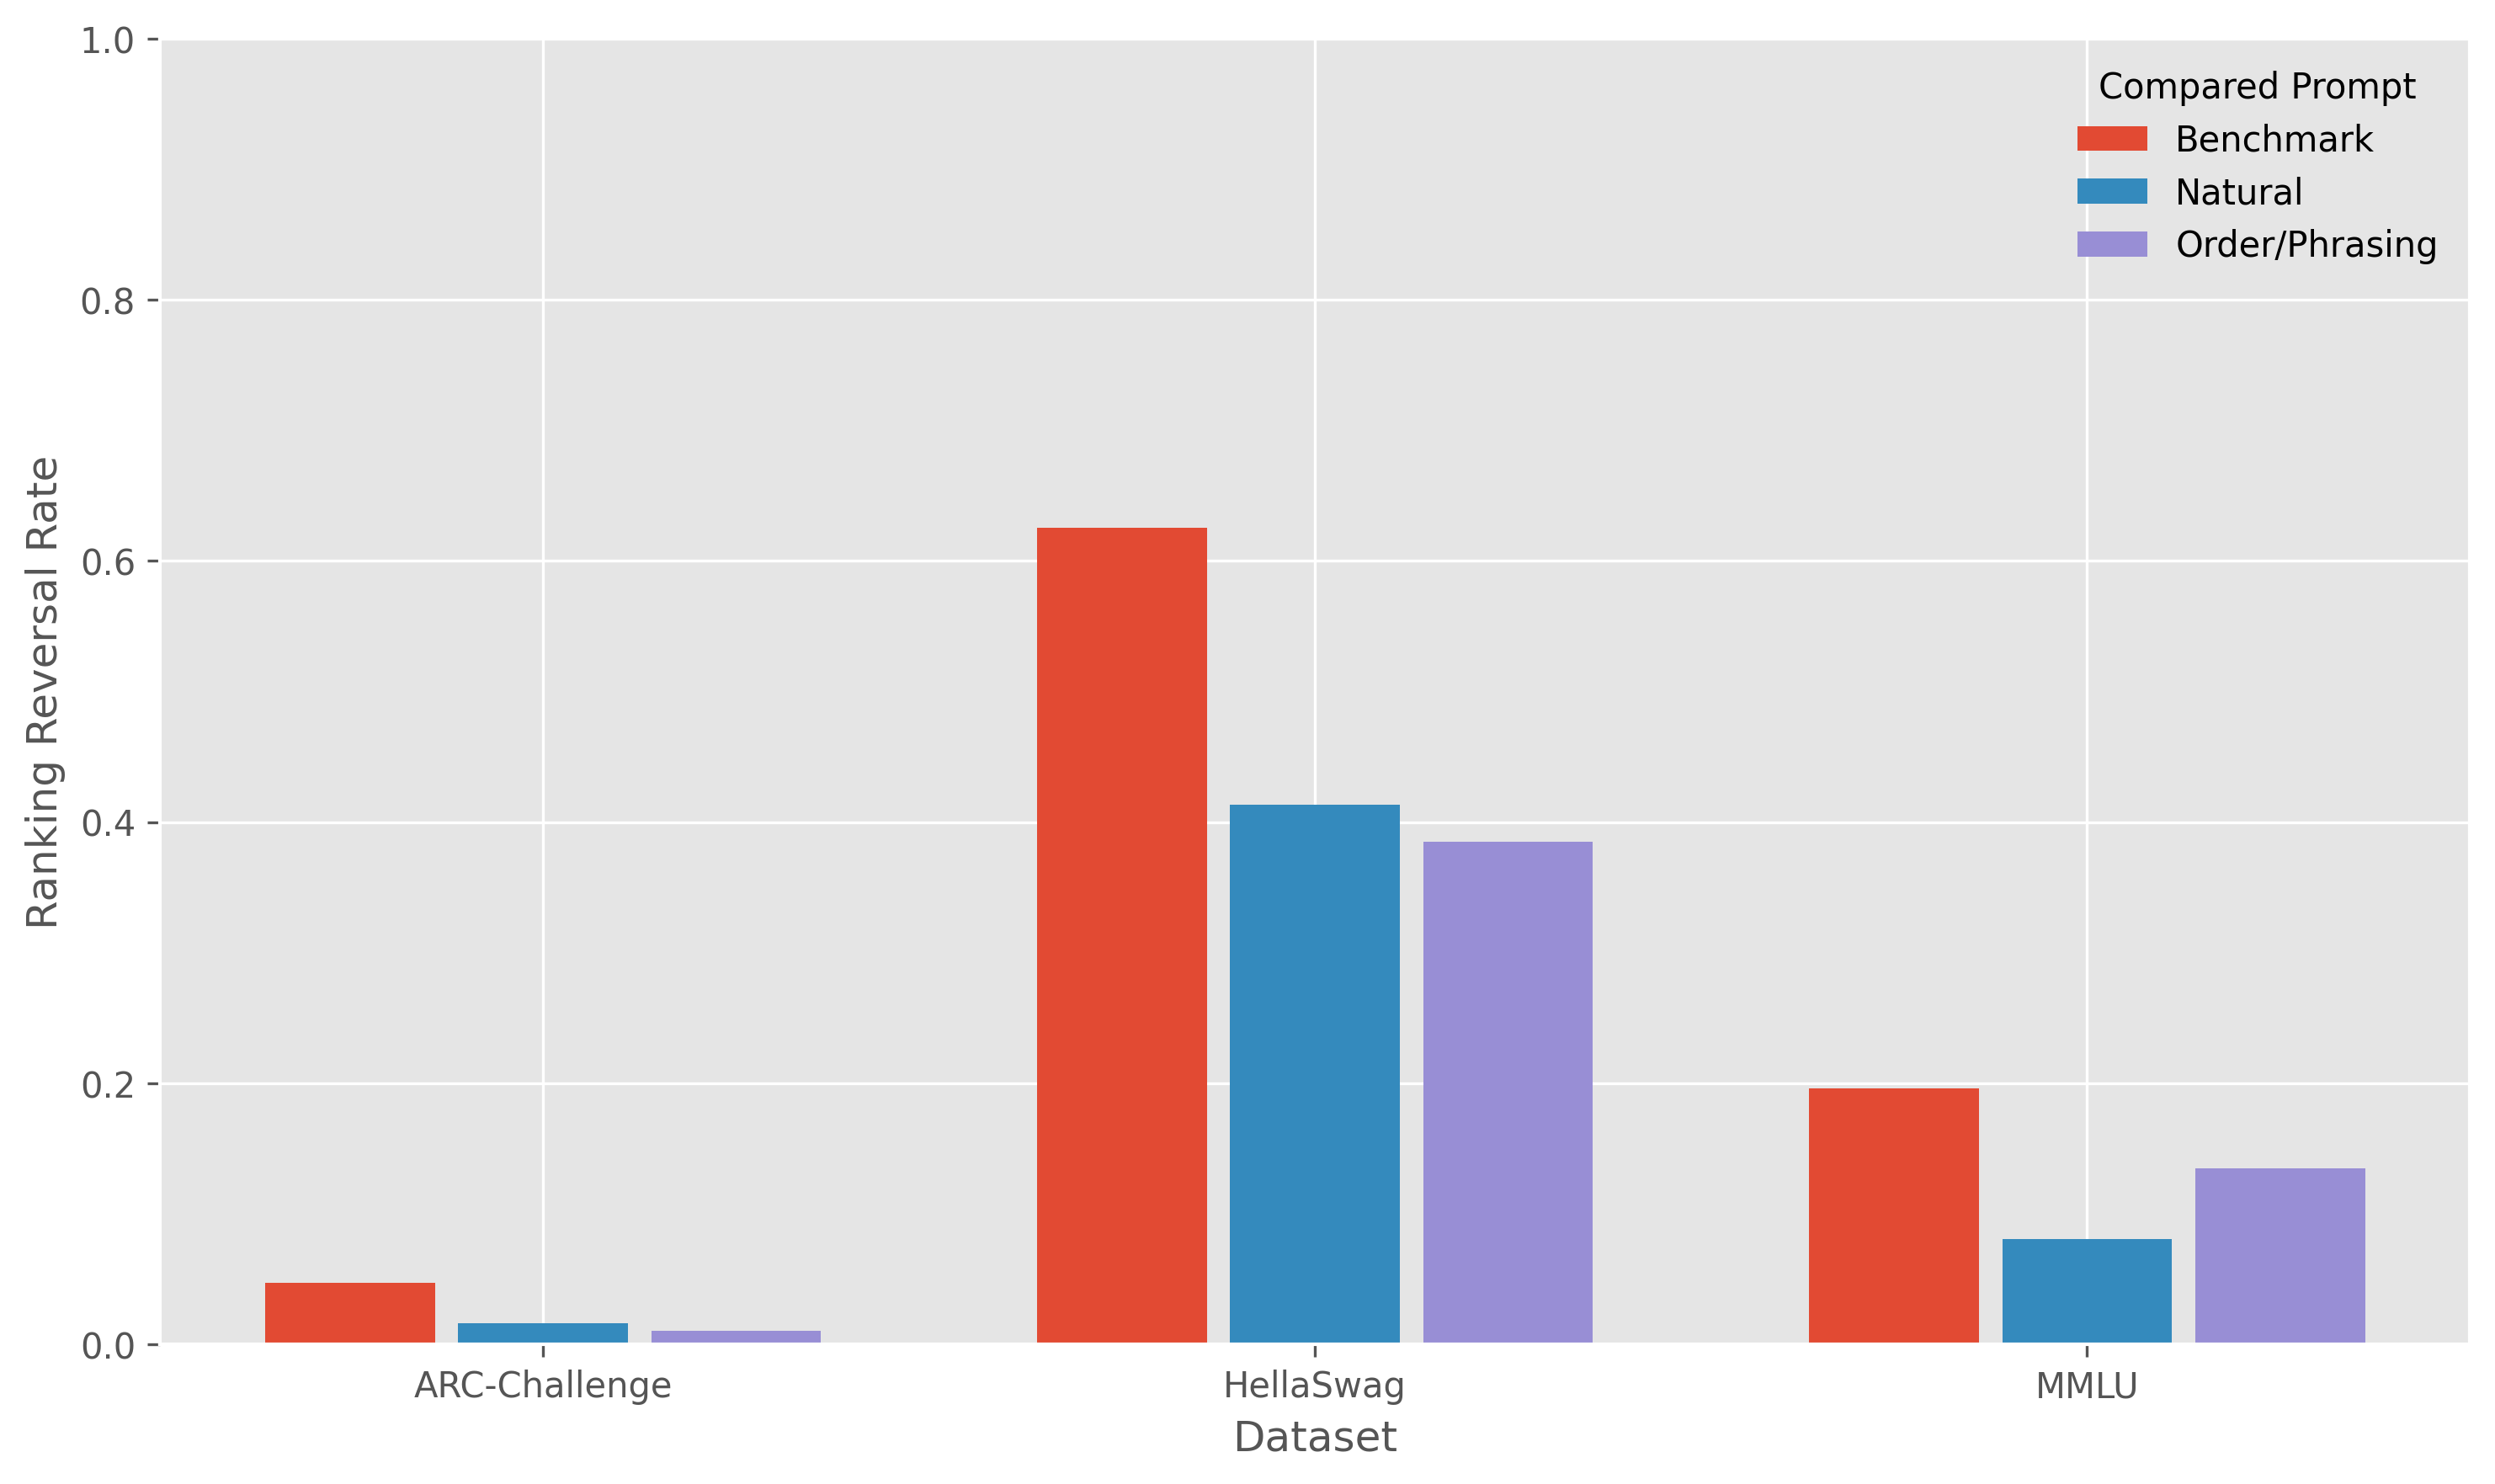
\includegraphics[width=\linewidth]{figures/ranking_reversal_rate.png}
    \column{0.34\textwidth}
    \only<2->{\numbercard{ARC}{RRR stays close to zero}}
    \vspace{0.25cm}
    \only<3->{\numbercard{MMLU}{stable winner, less stable middle}}
    \vspace{0.25cm}
    \only<4->{\numbercard{HellaSwag}{ranking flips surprisingly often}}
  \end{columns}
}

\appleframe{
  \vspace{1.0cm}
  \hero{HellaSwag is the wake-up call.}{The winner looks clear, until you ask whether it is actually stable.}
  \vspace{0.7cm}
  \begin{columns}[T,totalwidth=\textwidth]
    \column{0.32\textwidth}
    \only<1->{\numbercard{62.55\%}{highest ranking reversal rate}}
    \column{0.32\textwidth}
    \only<2->{\numbercard{1.92\%}{GPT lead over Gemini}}
    \column{0.32\textwidth}
    \only<3->{\numbercard{$p = 0.169$}{gap is not significant}}
  \end{columns}
  \vspace{0.9cm}
  \only<4>{
    \bigquote{Point estimate says GPT is first.}
  }
  \only<5>{
    \bigquote{Robustness analysis says the top rank is fragile.}
  }
}

\appleframe{
  \vspace{0.9cm}
  \hero{ARC is the opposite case.}{Sometimes the leaderboard really is robust.}
  \vspace{0.6cm}
  \begin{columns}[T,totalwidth=\textwidth]
    \column{0.58\textwidth}
    \only<1->{
      \begin{itemize}
        \item Gemini stays first under all prompt variants.
        \item All pairwise gaps are significant.
        \item Prompt and subset variation are too weak to overturn the order.
      \end{itemize}
    }
    \column{0.36\textwidth}
    \only<2->{\numbercard{94.00\%}{Gemini average accuracy}}
    \vspace{0.25cm}
    \only<3->{\numbercard{1--5\%}{RRR range only}}
  \end{columns}
  \vspace{0.8cm}
  \only<4>{
    \bigquote{Our claim is not that every leaderboard is unreliable.}
  }
}

\appleframe{
  \vspace{0.9cm}
  \hero{MMLU is more subtle.}{The top is stable. The middle is not.}
  \vspace{0.7cm}
  \begin{columns}[T,totalwidth=\textwidth]
    \column{0.56\textwidth}
    \begin{itemize}[<+->]
      \item Gemini remains clearly first.
      \item GPT vs Qwen is not significantly separated.
      \item So instability is concentrated in the middle ranks.
    \end{itemize}
    \column{0.36\textwidth}
    \only<2->{\numbercard{11.67\%}{Gemini lead over GPT}}
    \vspace{0.25cm}
    \only<3->{\numbercard{3.08\%}{GPT lead over Qwen}}
    \vspace{0.25cm}
    \only<4->{\numbercard{$p = 0.184$}{not significant}}
  \end{columns}
}

\appleframe{
  \vspace{0.8cm}
  \hero{And even MMLU is not uniform.}{Robustness also depends on the subject area.}
  \vspace{0.5cm}
  \begin{columns}[T,totalwidth=\textwidth]
    \column{0.62\textwidth}
    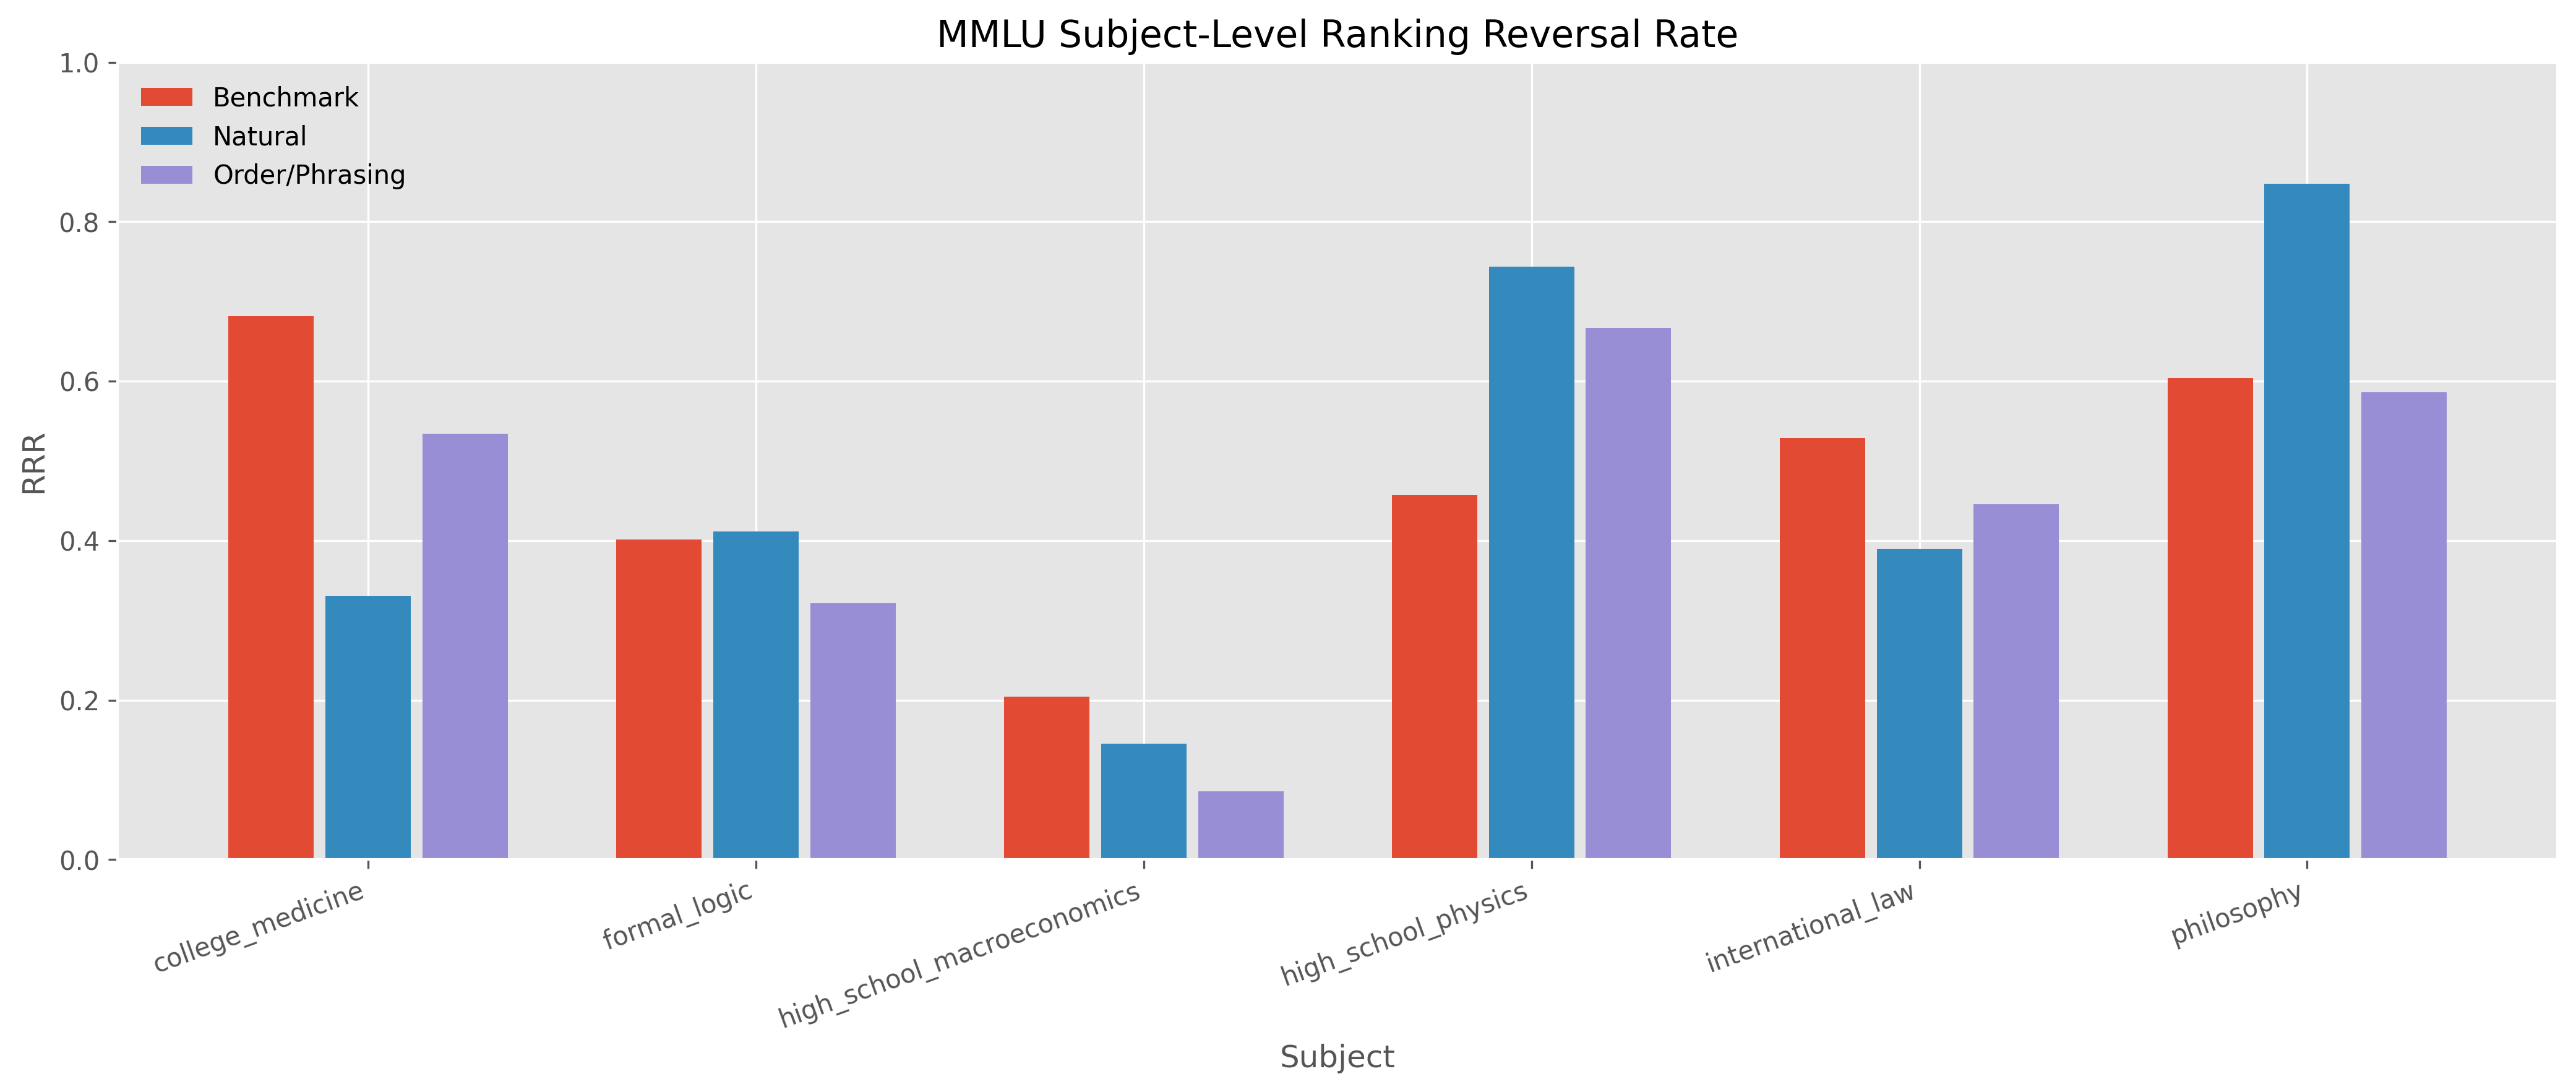
\includegraphics[width=\linewidth]{figures/mmlu_subject_rrr.png}
    \column{0.33\textwidth}
    \only<2->{
      \begin{itemize}
        \item Some subjects are relatively stable.
        \item Others show large prompt-driven rank changes.
      \end{itemize}
    }
    \vspace{0.35cm}
    \only<3->{\numbercard{14.5\%}{low end of mean subject RRR}}
    \vspace{0.25cm}
    \only<4->{\numbercard{67.9\%}{high end of mean subject RRR}}
  \end{columns}
}

\appleframe{
  \vspace{1.0cm}
  \hero{So what does the project actually show?}{A better way to read benchmark results.}
  \vspace{0.9cm}
  \begin{columns}[T,totalwidth=\textwidth]
    \column{0.31\textwidth}
    \only<1->{\numbercard{What we measured}{ranking stability, not just average score}}
    \column{0.31\textwidth}
    \only<2->{\numbercard{What we found}{robust, partially stable, and fragile leaderboards all exist}}
    \column{0.31\textwidth}
    \only<3->{\numbercard{What it implies}{uncertainty and robustness should be reported explicitly}}
  \end{columns}
}

\appleframe{
  \vspace{2.0cm}
  \bigquote{The real question is not only who is best.}
  \vspace{0.8cm}
  \only<2->{\bigquote{It is whether that ordering survives reasonable evaluation variation.}}
  \vfill
  \only<3->{\centering{\color{Muted}\large Thank you.}}
  \vspace{0.8cm}
}

\end{document}
